\chapter{Method}

\begin{enumerate}   \item Description of Node Copying as a method
  \begin{enumerate}     \item Node structure expansion
    \begin{enumerate}       \item Back pointers
      \item Modifications \item Bounds on numbers of the above \item How it
      works \item Why it works     \end{enumerate}
    \item Surrounding structure (collection of version information)
    \begin{enumerate}       \item Considerations about effecient storage and
    retrieval of version info     \end{enumerate}
  \end{enumerate}
  \item Description of ``Rollback'' as a method \begin{enumerate}     \item
  Description of reordering and optimization of operations (see algorithm
  \ref{alg:opsort} on page \pageref{alg:opsort})
  \end{enumerate}
  \item Definitions of various application profiles (how the DS is used)
  \end{enumerate}

\section{The Node Copying method}
Node Copying is a method described in \cite{Driscoll198986} by which a data
structure may be made partially persistent through the systematic expansion of
the nodes of the data structure. An auxillary data structure maintaining entry
points into the data structure, such as which node is the head of a linked list,
is also introduced. These two modifications of the data structure enable queries
to be made with $O(1)$ factor running time overhead and $O(1)$ space
consumption, given that the original data structure has an upper bounded
in-degree. In the following, I will describe in detail the general procedure as
well as giving the concrete example of the linked list.

\subsection{Node structure expansion}
As part of the Node Copying method, the node structure is expanded by adding two
arrays; one for ``back pointers'' and one for ``modifications''.

\begin{description}
  \item[Back pointers] 

  point back from a node $x$ to every node $y_i$ which points to $x$. When the
  in-degree has an upper bound, it is possible to restrict the size of the back
  pointers array. Whenever a node $y_i$ changes one of its pointers, the node
  $x$ it previously pointed to has the corresponding back pointer cleared, and
  the node $z$ it now points to has its corresponding back pointer set to point
  to $y_i$.

  \item[Modifications] store updates made to any of the fields of the node,
  including non-pointer fields, made since the node was created -- that is, the
  original field values from the time of construction remain unchanged. A
  modification record consist of a version number a field identifier and a
  value.

  When a field is to be modified on a node whose modifications array is already
  full, a copy of the node is constructed using the latest version of each field
  (including the one which is to be changed), thus resulting in a new node with
  an empty modifications array. The back pointers are also copied from the
  original node, and if the field being updated is a pointer field, the
  corresponding back pointer is updated in the destination node. This procedure
  is why the overall method is called Node Copying. A constant maximum number of
  modifications records is chosen such that node copying will have an amortized
  cost of $O(1)$.
\end{description}

\subsubsection{Amortized cost of Node Copying}
\todo[inline]{Write up proof of amortized time cost of node copying}

\section{Rollback}
Rollback is an approach to persistence based on the techniques described in
\cite{Tsotras1995237}, namely the combination of the na\"ive ``copy'' and
``log'' methods.
\subsection{The na\"ive approaches}
The ``copy'' approach makes a full copy of every version of the data structure
and makes it available by direct indexing to achieve $O(1)$ access overhead
factor. Creating each copy becomes more expensive in time and space the more
elements are inserted. In the worst case, when only insertions and no deletions
or modifications are made, the cost of creating $n$ versions is
$O\left(n^2\right)$.

The ``log'' approach conserves space by recording for each change made to the
data structure just enough information necessary to undo or redo it, thus giving
a space overhead factor per operation of $O(1)$. A ``current'' version
$v_{current}$ of the data structure is maintained. Given $v_{current}$, the
version $v_x$ can be produced by undoing or redoing all the changes between
$v_{current}$ and $v_x$ depending on which is the oldest. As the number of
versions $n$ increases, accessing a specific version becomes potentially more
costly. In the worst case, the overhead factor is $O(n)$ when $v_{current}$ is
$v_0$ and $v_x$ is $v_n$, or opposite.

\subsection{The hybrid approach}
An obvious hybrid of the two na\"ive approaches is to keep the records of each
operation like in the ``log'' approach, and storing a full copy like in the
``copy'' approach only at certain intervals. To access version $v_x$, the
nearest version to $v_x$ of which there exists a full copy, $v_s$, is retrieved.
Then, using the log of the versions from $v_s$ to $v_x$, the data structure
corresponding to $v_x$ is produced and returned.

Naturally, a user parameter is necessary to control the intervals at which full
copies are made. Let this parameter be $d$ and the number of versions $n$. There
will then be $\left\lfloor \frac{n}{d} \right\rfloor$ full copies, and the
maximum number of undos or redos to reach a specific version is then
$O(k+\frac{d}{2})$, where $k$ is the time required to retrieve the full copy. It
is now easy to see that the greater $d$ is, the fewer full copies will be made,
and thus the space cost is reduced accordingly. Likewise, the distance to the
version in the middle between two full copies increases with $d$, inducing a
higher cost for producing that version.

As an alternative to making a mutable copy of a full copy when a nearby version
is requested, one could instead allow the full copies to be mutable and moved
within $\pm\frac{d}{2}$ of their original location. This will increase the
maximum number of operations between a full copy and the desired version to $d$,
but will reduce greatly the time cost of making a working copy of the full copy.
If the full copies are originially uniformly distributed, direct lookup is still
possible, but it is then needed for each full copy to annotate which version it
represents.

\subsubsection{Adaptive copy interval increase}
It might be preferrable to be able to specify a space usage limit rather than a
fixed interval distance. When the space limit is near, $d$ is increased by a
factor $c$, and the existing full copies are discarded except from every $c$
copy, thus freeing up space for additional full copies.

\todo[inline]{Insert figure illustrating adaptive copy interval increase.}

\subsection{Operations sequence optimization}
For certain underlying data structures, it may prove to be feasible to
pre-process the sequence of operations between a full copy $v_s$ and the
requested version $v_x$ in order to reduce the actual work necessary to reach
$v_x$.

Two different types of pre-processing can be made to reduce work: Eliminating
superfluous operations and reordering operations. It is worth noting that both
of these require knowledge of the underlying data structure, and thus requires
more work to implement.

\subsubsection{Eliminating operations}
The sequence of operations between $v_s$ and $v_x$ may contain some operations
which will not need to be explicitly applied. The cases are:
\begin{enumerate}
  \item An \textsc{insert} operation followed by a \textsc{remove} operation at
  the same effective index -- both can be removed from the sequence since they
  cancel each other out.
  \label{item:elop-insert-remove}

  \item An \textsc{insert} operation followed by a \textsc{modify} operation at
  the same effective index -- the former can have its associated data value
  changed to that of the latter, and the latter can be removed from the
  sequence.
  \label{item:elop-insert-modify}

  \item A \textsc{modify} operation followed by a \textsc{remove} operation at
  the same effective index -- the former can be removed from the sequence.
  \label{item:elop-modify-remove}
\end{enumerate}

Cases \ref{item:elop-insert-remove} and \ref{item:elop-insert-modify} may of
course be combined in the sequence of one \textsc{insert} operation, one or more
\textsc{modify} operations and finally a \textsc{remove} operataion.


\paragraph{Algorithm.}
Pseudo code for an algorithm handling those cases is found in Algorithm
\ref{alg:eliminate-ops}.

\begin{algorithm}[p]
  \caption{An algorithm for eliminating superfluous operations}
  \label{alg:eliminate-ops}
  \begin{algorithmic}[5]
    \Procedure{EliminateSuperfluousOps}{sequence of operations $S$}
      \For {each operation $o_i \in S$, from last to first}
        \If {\textsc{type}($o_i$) $\in \left\{\textsc{insert},\textsc{modify}\right\}$}
        \State $c\gets\textsc{index}(o_i)$
          \For {each operation $o_j \in \left\{S|j>i\right\}$}
            \Switch {$\textsc{type}(o_j)$}
              \Case{\textsc{insert}}
                \If {$\textsc{index}(o_j) \le c$}
                  \State $c \gets c+1$
                \EndIf
              \EndCase
              \Case{\textsc{modify}}
                \If {$\textsc{index}(o_j) = c$}
                  \State $\textsc{data}(o_i) \gets \textsc{data}(o_j)$
                  \State remove $o_j$ from $S$
                \EndIf
              \EndCase
              \Case{\textsc{remove}}
                \If {$\textsc{index}(o_j) < c$}
                  \State $c \gets c-1$
                \ElsIf {$\textsc{index}(o_j) = c$}
                  \State $c \gets \textsc{index}(o_i)$
                  \Switch {$\textsc{type}(o_i)$}
                    \Case {\textsc{insert}}
                      \For {each operation $o_k \in \left\{S|i<k<j\right\}$}
                        \If {$\textsc{index}(o_k) > c$}
                          \State $\textsc{index}(o_k) \gets \textsc{index}(o_k) - 1$
                        \Else
                          \Switch {\textsc{type}($o_k$)}
                            \Case {\textsc{insert}}
                              \If {$\textsc{index}(o_k) \le c$}
                                \State $c \gets c+1$
                              \EndIf
                            \EndCase
                            \Case {\textsc{remove}}
                              \If {$\textsc{index}(o_k) \le c$}
                                \State $c \gets c-1$
                              \EndIf
                            \EndCase
                          \EndSwitch
                        \EndIf
                      \EndFor
                      \State remove $o_j$ from $S$
                      \State remove $o_i$ from $S$
                    \EndCase
                    \Case {\textsc{modify}}
                      \State remove $o_i$ from $S$
                    \EndCase
                  \EndSwitch
                \EndIf
              \EndCase
            \EndSwitch
          \EndFor
        \EndIf
      \EndFor
    \EndProcedure
  \end{algorithmic}
\end{algorithm}
 
The general idea is to identify cases \ref{item:elop-insert-remove},
\ref{item:elop-insert-modify} and \ref{item:elop-modify-remove} and make the
necessary maintenance before removing the relevant operations.

It iterates through the sequence backwards, i.e. from the last operation to the
first. If an \textsc{insert} or a \textsc{modify} operation $o_i$ is found, it
starts looking forwards for a matching \textsc{modify} or \textsc{remove}
operation. This is done by iterating through the proceeding operations while
keeping track of which index $c$ of the inserted or modified element would have
after each of the proceeding operations; if a proceeding operation $o_j$ inserts
or removes an element to the left of the originally inserted or modified
element, then the index would be shifted to the right or to the left,
respectively.

\newcommand{\specialcell}[2][c]{%
  \begin{tabular}[#1]{@{}l@{}}#2\end{tabular}}

If $o_j$ removes or modifies the element at index $c$, the type of $o_i$
determines what happens next. Table \ref{tab:oioj} shows which action is taken
depending on the types of $o_i$ and $o_j$.

\begin{table}[h]
  \center
  \begin{tabular}{|l|l|l|}\hline
    \diagbox{$o_i$\ \ }{$o_j$}&
    \textsc{modify} & \textsc{remove}\\
    \hline
    \textsc{insert} & update $o_i$ data, remove $o_j$ & \specialcell[t]{compensate between $o_i$ and $o_j$, \\ then remove both}\\
    \hline
    \textsc{modify} & update $o_i$ data, remove $o_j$ & remove $o_i$\\
    \hline
  \end{tabular}
  \caption{The table shows which action is taken depending on the types of $o_i$ and $o_j$.}
  \label{tab:oioj}
\end{table}

The compensation referred to in the case when $o_i$ is an \textsc{insert}
operation and $o_j$ is a \textsc{remove} operation works as follows:

\begin{itemize}

  \item Like in the iteration of the operations proceeding $o_i$, the index $c$
  of the inserted element is maintained while the operations between $o_i$ and
  $o_j$ (both exclusive) are iterated first to last.

  \item Since no operation prior to $o_j$ matches $o_i$, it is safe to assume
  that all operations between them have either greater or smaller indices than
  $c$. If the operation $o_k$ between $o_i$ and $o_j$ works on a smaller index,
  it will compensate the maintained index $c$ by -1 or +1. If $o_k$ works on a
  greater index, $o_k$ will itself have the index it works on reduced by 1,
  since its original index depended on the element of $o_i$ being inserted
  before it.
  
  \item When all operations between $o_i$ and $o_j$ have been examined thusly,
  $o_j$ and $o_i$ are removed from the sequence and the backwards iteration is
  resumed.
  
\end{itemize}

When the backwards iteration is finished examining the first operation in the
sequence, the algorithm terminates and the sequence now contains no operations
matching cases \ref{item:elop-insert-remove}, \ref{item:elop-insert-modify} or
\ref{item:elop-modify-remove}.

The space cost of the algorithm is in the order of the sequence size, i.e.
$O(\left|S\right|)$, since a mutable copy of the relevant operations is made.
In the worst case, when all $n$ operations are \textsc{insert} or
\textsc{modify} operations, the time cost is $O\left(n^2\right)$, since with
every \textsc{insert} operation, all the proceeding operations are examined when
a matching \textsc{remove} operation is not found.

\subsubsection{Reordering operations}

Applying each operation in the sequence separately is potentially a time
expensive approach. Consider the case when each operation inserts an element at
the end of a linked list; the bulk cost for $n$ insertions on a list of length
$l$ would be $O\left(\left(l+n\right)^2\right)$ if every operation begins by
iterating from the head of the list to the index of insertion.

It would indeed be more efficient to make the insertions in one straight
iteration of the linked list, which would cost $O(l+n)$ -- $l$ for reaching the
end of the list, $n$ for all the insertions. But this is only possible if the
the operations are ordered by non-decreasing index of application. If they are
not, they will have to first be reordered.

Reordering the sequence of operations by index of application requires some
maintenance. Consider the case when an \textsc{insert} operation $o_i$, which
has a small index of application, is moved to an earlier position in the
sequence than it had originally. Any operations which formerly preceeded $o_i$,
and which after the move will instead proceed it, should take into account the
additional element being inserted; if their index of application is greater than
that of $o_i$, it should be incremented by 1. If $o_i$ is a \textsc{remove}
operation, the index of application should instead be decreased by 1 on those
operations.

\paragraph{Algorithm.} Pseudocode for an algorithm implementing the above
approach is found in Algorithm \ref{alg:opsort}.

\begin{algorithm}[!ht]
  \caption{Algorithm for reordering a set of operations}
  \label{alg:opsort}
  \begin{algorithmic}[5]
    \Function {ReorderOperations}{sequence of operations $S$}
      \State $R \gets$ empty set
      \While {$S$ not empty}
        \State // Find left-most operation with minimum index of application
        \State $o_{min} \gets$ op. with minimum index of application
        \State $index_{min} \gets$ index in $S$ of $o_{min}$
        \State \textsc{remove} $o_{min}$ from $S$
        \State \textsc{append} $o_{min}$ to $R$
        \Statex
        \State // Compensate op.s which will now proceed rather than
        preceed $o_{min}$
        \If {$o_{min}$ is an \textsc{insert} op.}
          \For {each op. $o_i\in \left\{S | 0\le i<index_{min}\right\}$ }
            \State \textsc{index}($o_i$) $\gets$ \textsc{index}($o_i$) + 1
          \EndFor
        \ElsIf {$o_{min}$ is a \textsc{remove} op.}
          \For {each op. $o_i\in \left\{S | 0\le i<index_{min}\right\}$ }
            \State \textsc{index}($o_i$) $\gets$ \textsc{index}($o_i$) - 1
          \EndFor
        \EndIf
       \EndWhile
      \Statex
      \State \Return $R$
    \EndFunction
  \end{algorithmic}
\end{algorithm}

The space cost is linear in the number of operations being reordered. Consider
the worst case, when the operations are ordered with strictly decreasing indices
of application; the time cost is then $O\left(n^2\right)$, since the entire
remaining sequence would have to be searched for the minimum index of
application prior to the removal of that element.

If the operations are already ordered by non-decreasing index of application,
the algorithm only adds to the time cost, and so it may be worth checking that
the sequence requires reordering prior to running the algorithm. That can be
achieved in $O(n)$ time by testing whether each operation works on an index
equal to or greater than the previous one.

An example of the reordering of 10 operations by the algorithm is found in
figure \ref{fig:reorder-example}.

\begin{figure}[p]
  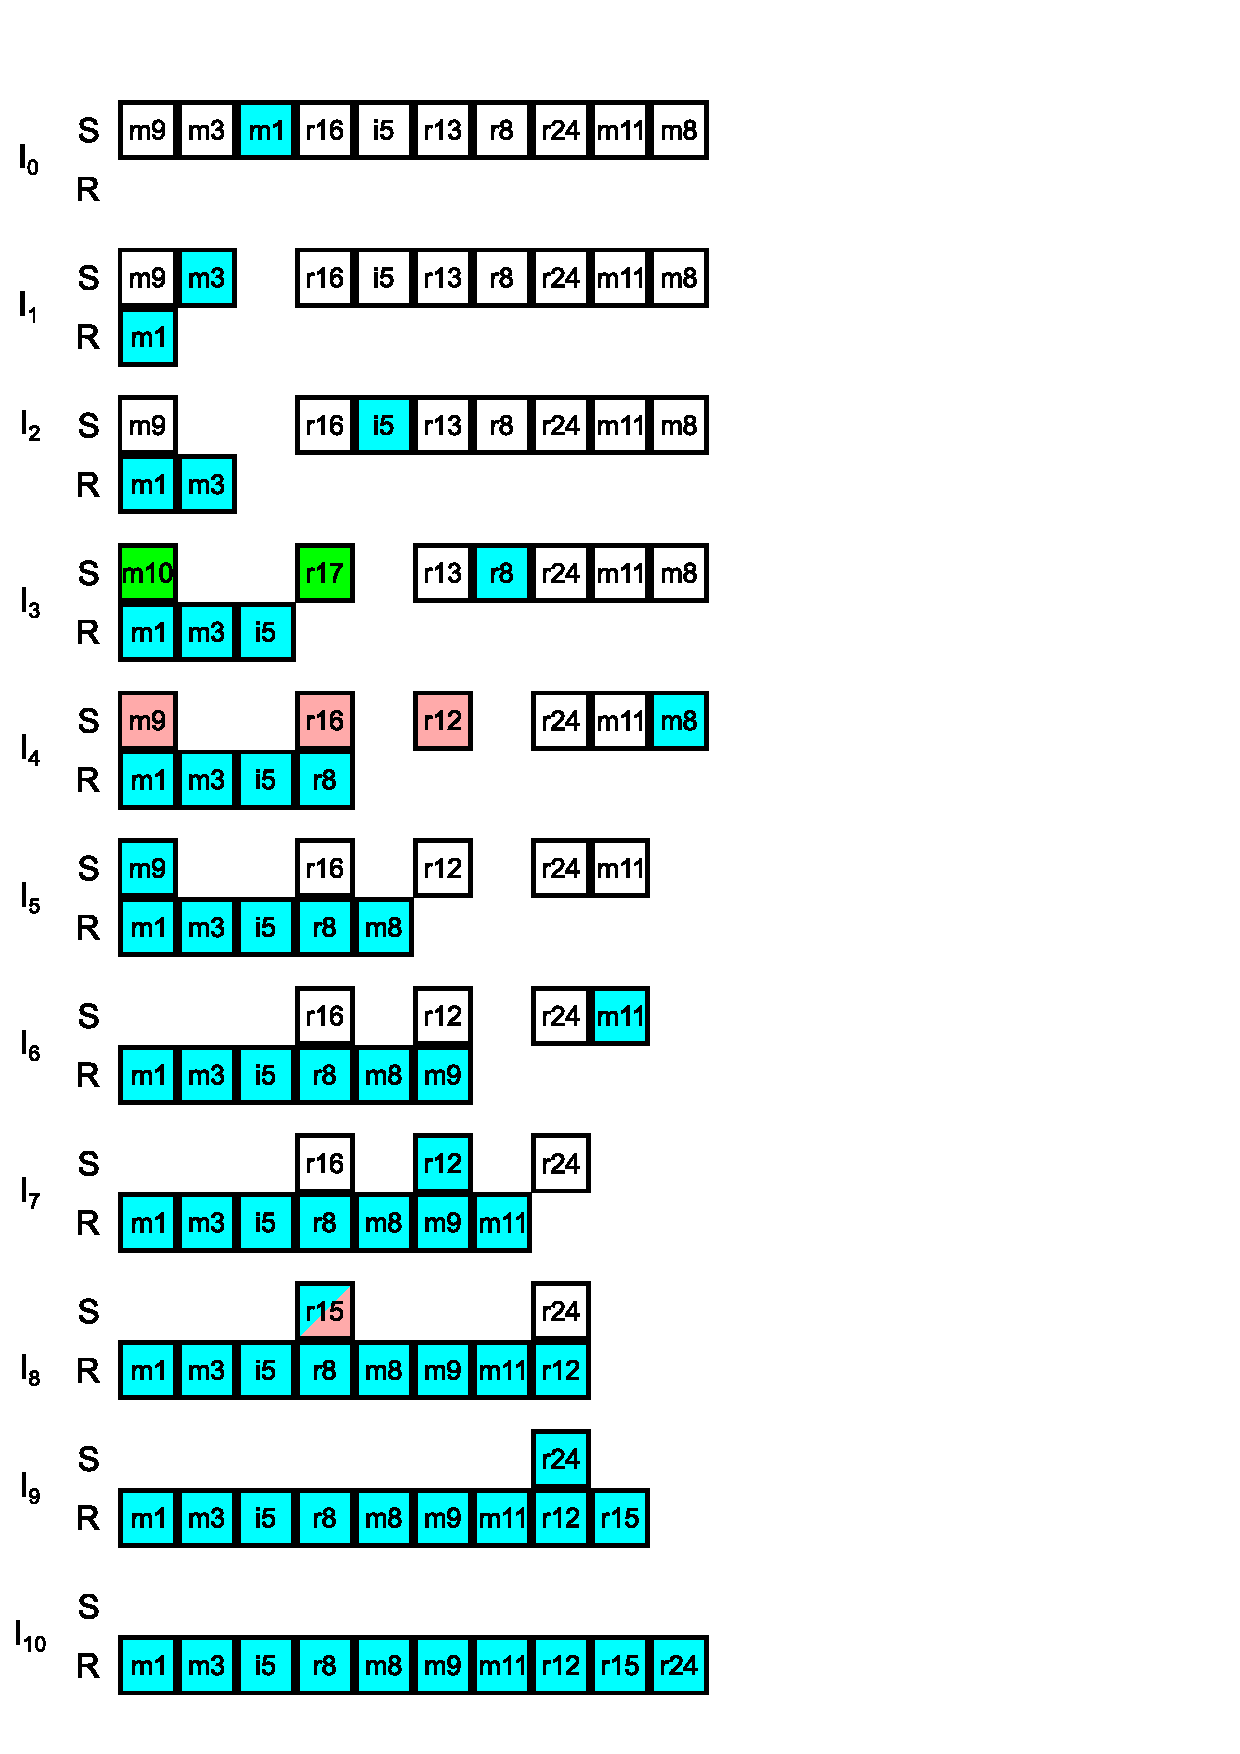
\includegraphics[width=.9\textwidth]{figures/reorder_example.pdf}

  \caption{\small Example of the reorder algorithm applied to a sequence of 10
  operations. In each iteration, the minimum operation in $S$ is colored cyan.
  When an \textsc{insert} operation is removed from $S$, the operations to the
  left are colored green to indicate the incrementation of their label.
  Similarly, when a \textsc{remove} operation is removed from $S$, the
  operations to the left are colored red to indicate the decrementation of their
  label.}

  \label{fig:reorder-example}
\end{figure}

\paragraph {Proof of reorder algorithm}
\begin{definition}
\label{def:reorder-iter}

Let $S_0$ be the original sequence given as input to the algorithm, and let
$O_0$ be an empty sequence at the beginning of the first iteration. By
definition, the sequence $O_0$, $S_0$ corresponds to (yields the same result as)
$S_0$. At the beginning of iteration $i$, let $l_{min_i}$ be the minimum index
of any operation in $S_i$, and let $o_{min_i}$ be the left-most operation in
$S_i$ with such index. Let $L_i$ be the operations to the left of $o_{min_i}$ in
$S_i$, and $R_i$ those to the right.

\end{definition}

\begin{lemma}
\label{lem:reorder-inequality}

By definition \ref{def:reorder-iter}, at the beginning of iteration $i$, all
operations in $L_i$ have greater indices than $o_{min_i}$, and no operations in
$R_i$ have smaller indices than $o_{min_i}$.

\end{lemma}

Since we intend to change the order of operations, consider the case of swapping
two operations. Let operation $o_b$ directly follow $o_a$ in a sequence. If
$o_b$ works on a smaller index than $o_a$, letting $o_b$ be applied before $o_a$
will potentially shift the elements in the list on which the operations work,
and $o_a$ will subsequently work on the wrong element unless compensation is
made.

Specifically, if $o_b$ is an \textsc{insert} operation, $o_a$ should be
compensated by incrementing by 1 the index on which it works, and by
decrementing it by 1 if $o_b$ is a \textsc{remove} operation. If $o_b$ is a
\textsc{modify} operation, it does not shift the elements in the list, and as
such nothing additional needs to be done after swapping the operations.

As a result, applying $o_a$, then $o_b$ corresponds to applying $o_b$, then the
compensated $o_a$.

Once $o_b$ has been swapped with $o_a$ and $o_a$ compensated, $o_b$ may again be
swapped with any operation to its left in a similar fashion, if that operation
also works on a greater index than $o_b$.

\begin{theorem}
\label{theorem:reorder-swap}

Any operation $o_b$ may be swapped with the immediately preceeding operation
$o_a$ if $o_a$ has a greater index of application. When $o_a$ is duly
compensated, the result will be the same.

\end{theorem}

If $o_{min_i}$ is swapped with each operation in $L_i$ -- which is possible by
taking into account lemma \ref{lem:reorder-inequality} and theorem
\ref{theorem:reorder-swap} -- it eventually ends up to the left of the
operations of $L_i$. Each of those operations would need compensation due to
working on greater indices than $o_{min_i}$.

Let
\begin{equation*}
  t_i = 
  \begin{cases}
      1, & \text{if $\textsc{type}(o_{min_i}) = \textsc{insert}$}.\\
      0, & \text{if $\textsc{type}(o_{min_i}) = \textsc{modify}$}.\\
      -1, & \text{if $\textsc{type}(o_{min_i}) = \textsc{remove}$}.
  \end{cases}
\end{equation*}

If we define $Lr_i$ as the same as $L_i$, except adding $t_i$ to the index of
each operation, then applying $L_i$, then $o_{min_i}$ corresponds to applying
$o_{min_i}$, then $Lr_i$.

Since the result of applying $o_{min_i}$, then $Lr_i$ corresponds to applying
$L_i$, then $o_{min_i}$, no operations in $R_i$ need adjustment.

\begin{theorem}
\label{thm:end-of-iter}

If, before the end of iteration $i$, $O_{i+1}$ is set to $O_i || o_{min_i}$ and
$S_{i+1}$ is set to $S_i \setminus \left\{o_{min_i}\right\}$, it follows that
applying $O_{i+1}$, then $S_{i+1}$ corresponds to applying $O_i$, then $S_i$.

\end{theorem}

\begin{proof}

Since in the end of each operation, the operation with the minimum index is
transferred from $S_{i-1}$ to the back of $O_i$, the operations in $O_i$ are
ordered by non-decreasing index. At the end of the last iteration, where
$i=\left|S_0\right|$, $S_i$ is empty and $O_i$ contains as many operations as
$S_0$, but in non-decreasing order of index of application. \qed

\end{proof}

When compared to the worst-case cost of applying the elements individually,
which is $O\left(\left(l+n\right)^2\right)$ for $n$ operations on an existing
list of length $l$, it is worth noting that only in the case of an empty list
and a long sequence of operations, the reordering algorithm is asymptotically as
slow. In all other cases, it is \emph{asymptotically} faster.
